\documentclass[conference]{IEEEtran}
\usepackage{cite}
\usepackage{amsmath,amssymb}
\usepackage{graphicx}
\usepackage{booktabs}
\usepackage{array}
\usepackage{url}
\usepackage{microtype}
\graphicspath{{figs/}}
\newcommand{\cm}{\,cm}

\begin{document}

\title{What to Share Depends on Sensing Quality:\\
A Preregistered Simulation Study of Cooperative Cable-Suspended Transport}

\author{\IEEEauthorblockN{Hao-Ting Ho}
\IEEEauthorblockA{Department of Electrical Engineering, Tunghai University, Taichung, Taiwan\\
haoting.ho@outlook.com}}

\maketitle

\begin{abstract}
Quadrotors carrying one cable-suspended payload can share teammates' \emph{geometry} (positions and rope directions) or their \emph{estimates} (measurements and information pairs for a consensus estimator). We ask which is worth sharing as onboard sensing degrades, in a preregistered MuJoCo study ($N{=}3$ quadrotors, distributed model predictive path integral (MPPI) control, 40 seeds $\times$ 2 trajectories $\times$ 5 sensing strengths $s$), with hypotheses, tests and decision rules frozen in an author-held git commit before the formal run. The answer depends on sensing quality but does not trend smoothly. With clean sensing ($s{=}0$) only the consensus estimator's gain is detectable. For $s\ge0.5$, teammate geometry gives a small detectable gain over a strong local extended Kalman filter (EKF) (mean paired payload-position RMSE difference $-0.38$ to $-0.67$\,cm, about 12--14\% of the EKF's RMSE, same sign throughout, no trend claimed). The overall gain of the consensus estimator over the geometry-augmented EKF (estimate exchange, payload center-of-mass offset $\delta c$ estimation and information-form filtering together, not separated) is detectable for $s\le1$ ($-0.16$ to $-0.64$\,cm), is largest at $s{=}0$ in point estimate, and for $s\ge1.75$ the evidence is insufficient (not shown to be absent). Across all five $s$ under ideal links, a consensus estimator truncated to 2 iterations and its centralized counterpart differ by at most 0.05\,cm, inside a preregistered $\pm0.25$\,cm band that is itself of the order of the other effects. All effects are millimetre-scale, from one simulator, team size and payload geometry; $-0.67$ is the figure-eight $s{=}2.5$ value with one failed episode scored by its raw RMSE (formal $-2.97$).
\end{abstract}

\begin{IEEEkeywords}
multi-robot transport, cable-suspended payload, distributed estimation, consensus, preregistration
\end{IEEEkeywords}

\section{Introduction}
In cooperative aerial transport with cables, each quadrotor feels only its own rope tension, yet the payload mass and center-of-mass offset are common to the team. The design question is \emph{what} to share. Teammates can broadcast pose and rope direction (\emph{geometry}), which determine the payload attitude and the load split among ropes. They can also exchange measurements and estimator information (\emph{estimates}) to estimate the shared payload parameters jointly. The two differ in cost, and a strong local estimator may already capture most of what either offers.

The work we reviewed does not compare the two. Decentralized payload control has estimated load share locally without estimate exchange~\cite{gpac2026} or targeted computation and communication load~\cite{tasooji2025} (Sec.~\ref{sec:related}). We did not find a study comparing geometry sharing against estimate sharing for cable-suspended transport across sensing quality; the search was limited, so this is no priority claim.

We therefore ask which is worth sharing as onboard sensing degrades, in simulation and against a tuned local EKF. The comparison is \emph{preregistered}: hypotheses, sensing grid, metric, tests and decision rules were frozen before the formal run (Sec.~\ref{sec:protocol} states what the freeze does not guarantee). With a strong base the answer differs by sensing regime without a smooth trend, and every effect is millimetre-scale (about 0.2--0.65\,cm); the contribution is the protocol and the decomposition of \emph{what} is shared, not a large improvement.

\textbf{Contributions.}
\begin{itemize}
\item A decomposition separating teammate \emph{geometry} from the consensus estimator (which adds estimate exchange, $\delta c$ estimation and an information-form filter), on a local EKF (EKF-L) base (Table~\ref{tab:info}).
\item A preregistered sweep over a sensing-strength scale $s$ with paired sign-flip tests, Holm correction and TOST equivalence.
\item Findings at measured size: geometry helps EKF-L for $s\ge0.5$ (about 0.4--0.65\,cm, no trend claimed); the consensus estimator helps on top of it for $s\le1$ (insufficient evidence above); under ideal links it is within 0.25\,cm of its centralized counterpart.
\item What the numbers do and do not support, including a failure-scoring artifact.
\end{itemize}

\section{Related Work}\label{sec:related}
GPAC~\cite{gpac2026} lists distributed fusion across cables as future work; event-triggered distributed NMPC~\cite{tasooji2025} targets computation and communication load. Center-of-gravity estimation has been studied for rigidly coupled drones~\cite{barawkar2024}, and cooperative payload-parameter estimation by multiple quadrotors in~\cite{arab2021} (full text not read). Consensus on parameter estimates is a general tool~\cite{mendez2026}; we use the hybrid consensus-on-measurements-and-information (HCMCI) scheme~\cite{battistelli_hcmci}. Background: cable-suspended load control~\cite{sreenath2013,lee2018,lee2013multi,sreenath_kumar2013,michael2011}, MPPI~\cite{williams2017}, MuJoCo~\cite{todorov2012}, Holm correction~\cite{holm1979}, TOST~\cite{schuirmann1987}. The search behind our gap statement (Sec.~I) was web search without citation tracking.

\section{Problem Setup and Methods}
\subsection{Plant and control}
\begin{figure}[t]
\centering
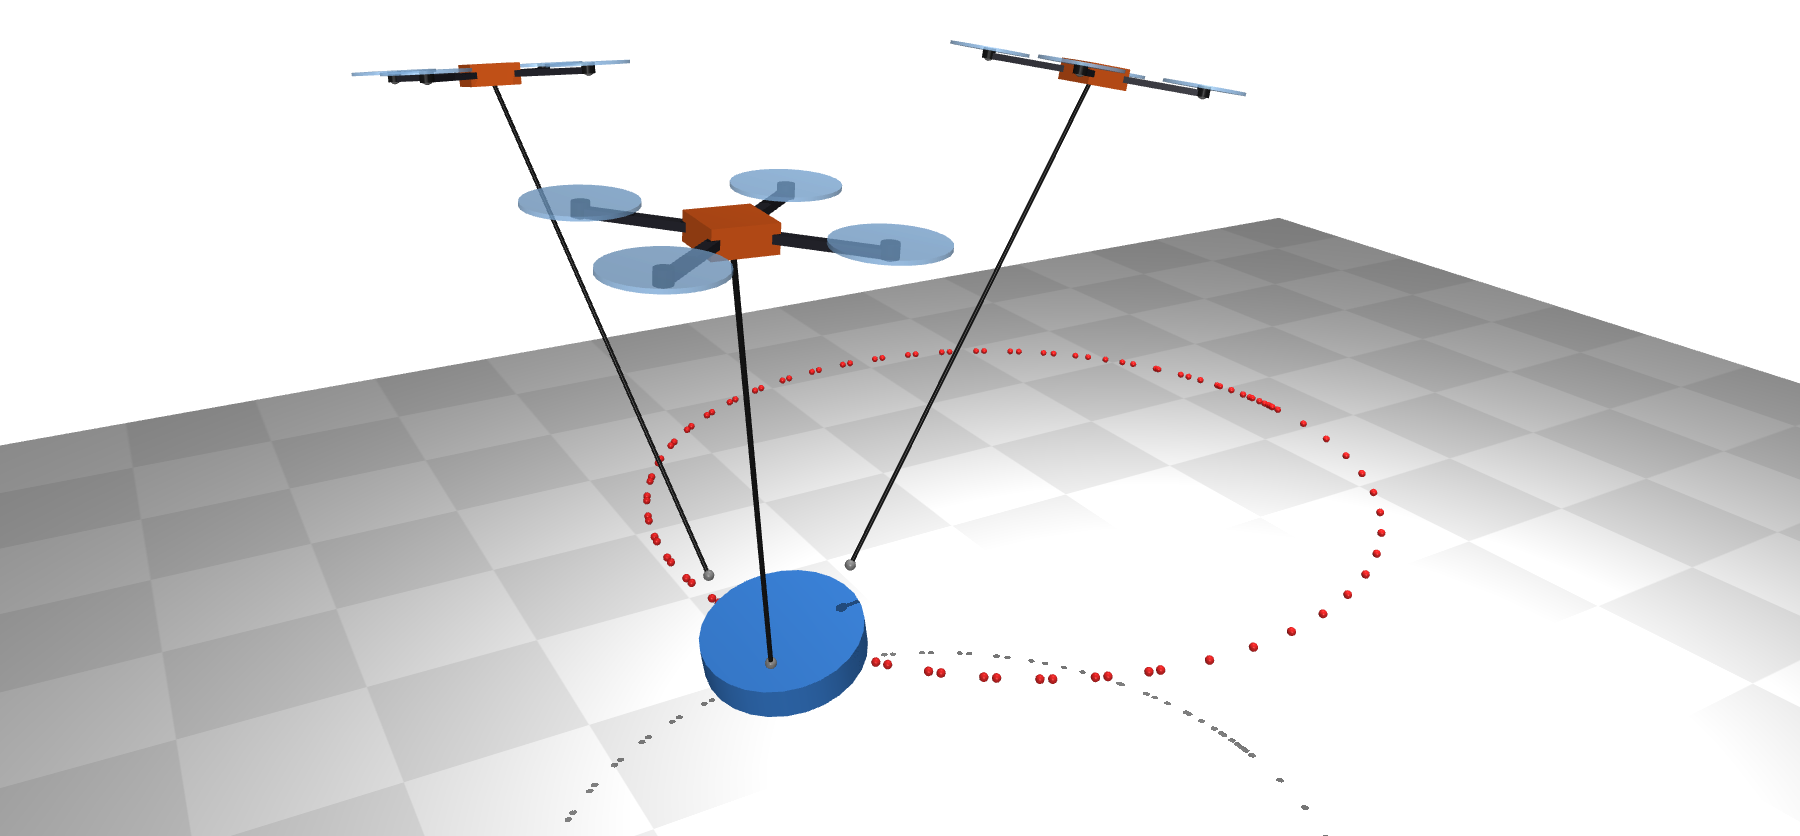
\includegraphics[width=0.6\columnwidth]{sim_snapshot_t4.png}
\caption{MuJoCo scene (CON-ATT, $s{=}1$, circle, $t{=}4$\,s); red: payload reference.}
\label{fig:scene}
\end{figure}
$N{=}3$ quadrotors (Fig.~\ref{fig:scene}; 1\,kg each) carry a payload (nominal 1\,kg, radius 0.15\,m) on 1\,m ropes in MuJoCo (control step 0.01\,s). The payload has an unknown mass offset $\delta m\in[-0.3,0.4]$\,kg and center-of-mass offset $\delta c$ (radius $\le0.04$\,m), and each agent has an unknown thrust-coefficient error $k_i$; $\theta_s=(\delta m,\delta c)$ is shared by the team while $\zeta_i=k_i-1$ is local. Every agent runs MPPI ($K{=}512$ samples, horizon 20 steps at 0.05\,s) with one hyper-parameter set frozen before this study and shared by all methods, so methods differ only in the estimator. Each agent feeds its own $\hat\theta_i$ into its MPPI payload model and divides its commanded thrust by $1{+}\hat\zeta_i$ (DOB does neither). Teammate information enters only through the estimator: geometry in its measurement model, consensus pairs in its state. Trajectories are a circle (radius 0.8\,m, 1.2\,rad/s) and a figure-eight (0.8\,m $\times$ 0.4\,m, 0.9\,rad/s), 10\,s long, no wind. Agents' onboard estimators never read payload ground truth.

\subsection{Sensing strength $s$}
Sensing quality is scaled by a single number $s$ (the values are assumed, not measured). IMU noise, IMU bias, thrust-coefficient error, and rope-direction noise interpolate linearly from the ``clean'' profile ($s{=}0$) to a ``moderate'' profile ($s{=}1$) and extrapolate beyond (e.g.\ IMU $\sigma$: $0.15+0.45s$\,m/s$^2$; bias std $0.1s$\,m/s$^2$; $k_i\sim U(1\pm0.05s)$). Measurement delay is a step function (0 steps for $s<0.5$, 2 for $s<1.75$, 3 otherwise, at 0.01\,s), and position noise is $0.01\min(s,1)$\,m. We evaluate $s\in\{0,0.5,1,1.75,2.5\}$; $s$ is therefore not a single linear scale.

\subsection{Methods and information}
Table~\ref{tab:info} lists what each estimator reads. ``Teammate geometry'' means teammate position and rope direction: with them, an agent recovers payload attitude by a Kabsch fit and replaces nominal rope tension allocation by an attitude-aware one. It is shared by the architecture, not agreed on by consensus.

\begin{table}[t]
\centering
\caption{Methods $\times$ information read by each agent's estimator. Relay: $N{-}1$ forwarding rounds on a path graph. Ideal links unless stated.}
\label{tab:info}
\footnotesize
\setlength{\tabcolsep}{2.5pt}
\begin{tabular}{lcccccc}
\toprule
Method & IMU & own & rope & team. & team. & team. \\
 & & pose & dir. & geom. & est. & meas. \\
\midrule
DOB & own & -- & -- & -- & -- & -- \\
LOC-M & own & \checkmark & \checkmark & -- & -- & -- \\
EKF-L & own & \checkmark & \checkmark & -- & -- & -- \\
EKF-L+GEO & own & \checkmark & \checkmark & relay & -- & -- \\
CON-ATT & own & \checkmark & \checkmark & relay & consensus & relay \\
CEN-ATT & team & \checkmark & \checkmark & central & central & central \\
\bottomrule
\end{tabular}
\end{table}

\emph{DOB}: low-pass filter of the force residual, no model feed-forward. \emph{LOC-M}: local recursive estimate of $\delta m$ plus $\hat\zeta_i$. \emph{EKF-L}: per-agent EKF with state $[\delta m,\zeta_i,b_i]$ where $b_i\in\mathbb{R}^3$ is the IMU bias (random-walk model), $\delta c$ fixed at 0. \emph{EKF-L+GEO}: EKF-L plus teammate geometry in the measurement model ($\delta c$ is not estimated in the frozen configuration); no torque pseudo-measurement, since that needs teammates' measurements. \emph{CON-ATT}: each agent keeps an information pair $(\Lambda_i,\xi_i)$ over the full team state $[\delta m,\delta c,\zeta_{1..N}]$ and runs HCMCI with Metropolis weights, 2 consensus iterations per step on a path graph (1--2--3); packets of teammates' $(p_q,q,y,f,\text{active})$ are relayed $N{-}1$ rounds. With ideal links every agent therefore holds the same data as the centralized \emph{CEN-ATT}, so any CON--CEN gap comes from truncated consensus only. For a dropped message (CON-ATT only; this applies to the relay rounds as well as the consensus iterations) the weight returns to the receiver; stale packets older than 5 steps trigger a fallback to nominal geometry. EKF-L+GEO does not implement dropout.\par
\emph{What H1b contains.} CON-ATT and EKF-L+GEO differ in three ways beyond estimate exchange: (a) CON-ATT is an information-form consensus filter, GEO an EKF; (b) CON-ATT estimates $\delta c$, GEO is frozen with \texttt{use\_dc}$=0$ (\texttt{results/p2d/best.json}); (c) their tuning budgets differ (Sec.~\ref{sec:protocol}). We therefore read H1b as the \emph{overall} gain of CON-ATT over GEO (estimate exchange, $\delta c$ estimation and information-form filtering together), not as the effect of estimate exchange alone.

\section{Preregistered Protocol}\label{sec:protocol}
\textbf{What the freeze means.} The freeze is a git commit (\texttt{5dd3cf7}, version v3, with the analysis script) in the authors' private repository; the public \texttt{docs/PREREG.md} is identical to it; there is no third-party timestamp. The formal run used fresh seeds (3000--3039), pilot data were declared not to count as evidence, and no deviation from the frozen protocol occurred. The authors had seen pilot data (seeds 2200--2219, also 2020--2029 and 2100--2119) before freezing. The rule that a failed episode is scored 100\,cm was set \emph{after} the pilot (the PREREG section on differences from the pilot: the pilot code scored only non-finite or $>1$\,m episodes as 1\,m). This rule is the source of the H2 magnitudes and of the fig8 artifact below; the sensitivity analysis with the pilot rule is reported.

\textbf{Primary metric.} $\mathrm{RMSE}_\text{eff}$: payload-position RMS error (cm) over the episode; an episode with non-finite values, $\text{success}=$ False, or RMSE $>1$\,m is scored 100\,cm. Success means last-second mean error $<0.10$\,m and maximum error $<0.5$\,m. Failed episodes are never dropped.

\textbf{Hypotheses} (differences are A$-$B, negative is better; analysed per trajectory, paired by seed, 40 seeds).
\begin{itemize}
\item \textbf{H1a:} $D_a(s)=$ RMSE(EKF-L+GEO) $-$ RMSE(EKF-L) $<0$.
\item \textbf{H1b:} $D_b(s)=$ RMSE(CON-ATT) $-$ RMSE(EKF-L+GEO) $<0$ (overall gain of CON-ATT over GEO, an increment on top of geometry, not an additive decomposition and not a pure estimate-exchange effect, see Sec.~III-C).
\item \textbf{H2:} the OLS slope in $s$ of $B_\text{DOB}(s)=$ RMSE(DOB) $-$ RMSE(CON-ATT) is positive.
\item \textbf{H3:} CON-ATT and CEN-ATT are equivalent within $\pm0.25$\,cm at $s{=}1$ (TOST; $\pm0.5$\,cm as sensitivity).
\item \textbf{H4} (secondary): the slope of $D_a-D_b$ in $s$ is negative (direction only; not used for the main claim).
\end{itemize}

\textbf{Statistics.} One-sided paired sign-flip permutation tests ($10^5$ flips), Holm correction within preregistered families (F1: H1a and H1b $\times$ 5 $s$ $\times$ 2 trajectories, 20 tests; F2: H2; F3: H3; further secondary families), $\alpha=0.05$; 95\% percentile-bootstrap CIs over seeds (10\,000 resamples). A $(\text{hypothesis},s)$ cell is ``\emph{supported}'' only if \emph{both} trajectories are rejected after Holm; otherwise it is ``insufficient evidence'' (not ``no effect'': equivalence was tested only for H3). A practical threshold $\Delta=0.5$\,cm is descriptive: a cell ``reaches $\Delta$'' if both mean differences are $\le-0.5$\,cm.

\textbf{Tuning.} All hyper-parameters were tuned once, at $s{=}1$, speed 1.0, on separate seeds (2020--2024) and then frozen. GEO was tuned after the other methods (PREREG \S3.3). The budget (PREREG \S3.3) was asymmetric: 14 grid points for EKF-L, 10 for EKF-L+GEO, 10 for LOC-M, 9 for CEN-ATT (shared by CON-ATT), 8 for DOB; each point was evaluated on only 10 episodes (5 seeds $\times$ 2 trajectories). EKF-L's extra points were a recorded extension (a deviation from the P2d specification, disclosed in the PREREG). The extra budget favours EKF-L, so the direction is conservative for the geometry claim (H1a), but GEO (10) and CON-ATT (9) are close, so it does not hold for H1b.

\section{Results}
\subsection{H1: what to share, by $s$}
Table~\ref{tab:h1} and Fig.~\ref{fig:h1} give the per-$s$ results, with means and, in parentheses, medians of the paired differences (the median is needed because mean-based thresholds can be met while the median is not).

\begin{table}[t]
\centering
\caption{Paired RMSE$_\text{eff}$ differences in cm, mean (median), 40 seeds, A$-$B. $D_a$: EKF-L+GEO $-$ EKF-L; $D_b$: CON-ATT $-$ EKF-L+GEO. Italic: not rejected after Holm (F1). $\dagger$: see text.}
\label{tab:h1}
\footnotesize
\setlength{\tabcolsep}{3pt}
\begin{tabular}{lcccc}
\toprule
 & \multicolumn{2}{c}{$D_a$ (H1a)} & \multicolumn{2}{c}{$D_b$ (H1b)} \\
$s$ & circle & fig8 & circle & fig8 \\
\midrule
0 & \textit{+0.12 (--0.06)} & \textit{--0.05 (--0.16)} & --0.64 (--0.27) & --0.52 (--0.14) \\
0.5 & --0.38 (--0.38) & --0.47 (--0.35) & --0.25 (--0.12) & --0.21 (--0.13) \\
1 & --0.38 (--0.21) & --0.42 (--0.20) & --0.16 (--0.10) & --0.20 (--0.17) \\
1.75 & --0.50 (--0.33) & --0.51 (--0.25) & \textit{--0.16 (--0.03)} & \textit{--0.20 (--0.12)} \\
2.5 & --0.65 (--0.38) & --2.97$^\dagger$ (--0.45) & \textit{--0.19 (--0.09)} & \textit{--0.23 (--0.10)} \\
\bottomrule
\end{tabular}
\end{table}

\begin{figure}[t]
\centering
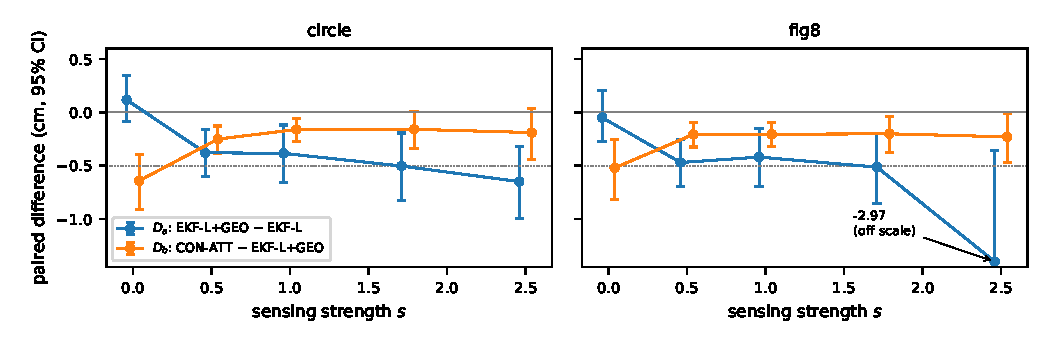
\includegraphics[width=\columnwidth]{fig_H1.pdf}
\caption{$D_a$ and $D_b$ (mean, 95\% bootstrap CI) versus $s$; dotted line $-\Delta=-0.5$\,cm. Formal values, with the lower end of the fig8 $s{=}2.5$ interval clipped; that point is dominated by one failed EKF-L episode (see text).}
\label{fig:h1}
\end{figure}

\textbf{Geometry (H1a).} For $s\ge0.5$ H1a is supported on both trajectories, with mean differences from $-0.38$ to $-0.65$\,cm (about 12--14\% of EKF-L's RMSE; Holm-adjusted $p$ from $0.001$ to $0.033$), same sign throughout, no trend claimed. We quote this range ($-0.38$ to $-0.65$) for the non-artifact cells throughout; the abstract's $-0.67$ is fig8 $s{=}2.5$ under the raw-RMSE sensitivity rule (formal $-2.97$, below). For $s=0$ the evidence is insufficient ($+0.12$ and $-0.05$\,cm, CIs include 0). Mean differences are about $-\Delta$ at $s=1.75$ ($-0.503$, $-0.513$); medians are above $-0.5$\,cm everywhere ($-0.20$ to $-0.45$ for $s\ge0.5$), so ``reaches $\Delta$'' concerns the mean only.

\textbf{CON-ATT over EKF-L+GEO (H1b).} For $s\le1$ H1b is supported on both trajectories ($-0.16$ to $-0.64$\,cm; only $s=0$ reaches $\Delta$, with medians $-0.27$ and $-0.14$\,cm). The point estimate is largest at $s=0$ and similar from $0.5$ to $1$; the $s=0$ versus $0.5$ difference was not tested, and it coincides with the delay jump from 0 to 2 steps. For $s=1.75$ and $2.5$ the evidence is insufficient: no cell passes Holm (adjusted $p$ 0.07--0.21) and the preregistered power there was low (about 0.1). This is not evidence of no effect.

\textbf{Reading the two together.} We describe three regimes and no trend. At $s=0$ only the estimator gain is detectable (geometry: insufficient evidence). For $s\ge0.5$ the geometry gain is detectable with the same sign, about 0.4--0.65\,cm, no trend claimed. The estimator gain is largest at $s=0$ in point estimate (see above) and is not established for $s\ge1.75$. We do \emph{not} claim that the gain ``shifts'' to geometry as sensing degrades. The secondary H4 test has a negative circle slope of $D_a-D_b$ ($-0.40$\,cm per unit $s$, adjusted $p=0.0004$); we claim only the direction. The circle slope is set mainly by the $s{=}0$ end point (excluding $s{=}0$ it is $-0.17$). The fig8 formal slope ($-1.07$, $p=0.0029$) is produced by the failed episode described next; with failed episodes scored by raw RMSE (sensitivity (a)) it is $-0.28$, and $-0.096$ if $s{=}0$ is also dropped (\texttt{paper/\allowbreak workshop/\allowbreak scripts/\allowbreak recompute\_h4\_sens.py}). We therefore do not rely on the fig8 $p$-value.

\textbf{One failed episode.} At $s{=}2.5$, fig8, EKF-L seed 3024 has RMSE 7.9\,cm but \texttt{success=False}, hence is scored 100\,cm. This produces the formal $D_a=-2.97$\,cm (fig8), the total CON-ATT $-$ EKF-L gain of $-3.20$\,cm, and the H4 fig8 slope of $-1.07$. Under the preregistered sensitivity analysis that scores failed episodes by their raw RMSE (when $\le 1$\,m), the fig8 $D_a$ at $s{=}2.5$ is $-0.67$\,cm (90\% CI $-0.96$ to $-0.38$); this is the value we use in the discussion. The other 19 H1 cells are unchanged.

\subsection{H2: gain over a simple local method}
The preregistered slope of $B_\text{DOB}(s)$ is positive on both trajectories (formal $+11.0$ and $+10.6$\,cm per unit $s$, adjusted $p<10^{-4}$), and the slope is positive for all 40 seeds. \emph{These magnitudes are an artifact of the 1\,m failure scoring}: DOB fails in 22 of 80 episodes at $s{=}2.5$ (success 58/80; per trajectory 0.70 [0.55,0.82] and 0.75 [0.60,0.86], Wilson 95\%), versus 80/80 for CON-ATT. Using raw RMSE the slope is $+1.84$ (circle) and $+1.90$\,cm per unit $s$, with raw $B_\text{DOB}$ rising from $0.4$\,cm and $0.2$\,cm at $s{=}0$ to $4.95$ and $4.92$\,cm at $s{=}2.5$ (Fig.~\ref{fig:h2}). Caveats: (i) $s$ is not linear, so the slope is a coarse summary; (ii) DOB's cutoff was tuned at $s{=}1$ and DOB applies no $\hat\zeta$ compensation, so the comparison mixes ``shared estimation'' with ``model feed-forward plus compensation''; (iii) the secondary LOC-M slope is also positive (formal $+1.34$, $+2.89$, same caveat), and LOC-M itself fails 4 episodes at $s{=}2.5$.

\begin{figure}[t]
\centering
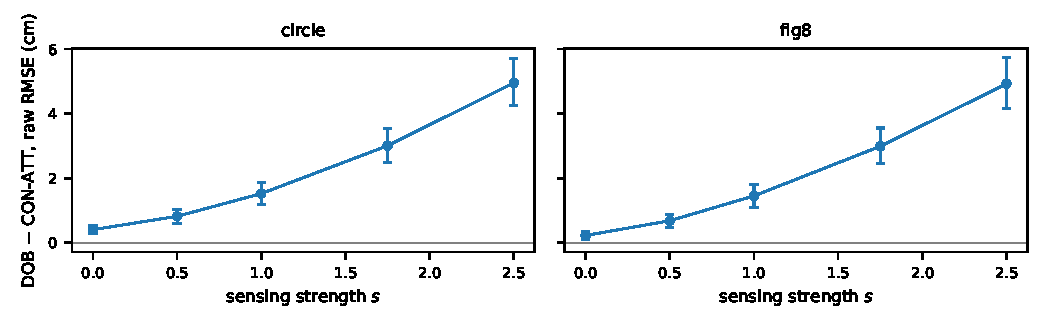
\includegraphics[width=\columnwidth]{fig_H2_raw.pdf}
\caption{$B_\text{DOB}(s)=$ RMSE(DOB) $-$ RMSE(CON-ATT) on the \emph{raw} payload RMSE (cm), mean with 95\% bootstrap CI over 40 seeds (recomputed from the episode file for this figure). The preregistered metric scores failed episodes as 100\,cm and gives values of 31.9 and 27.2\,cm at $s{=}2.5$.}
\label{fig:h2}
\end{figure}

\subsection{H3: distributed versus centralized}
CON-ATT $-$ CEN-ATT at $s=1$ is $-0.021$\,cm (circle) and $-0.033$\,cm (fig8); the 90\% CIs are $[-0.032,-0.010]$ and $[-0.043,-0.023]$\,cm. Both TOST tests pass at $\pm0.25$\,cm (adjusted $p<10^{-4}$) and also at all four other $s$ (means from $-0.049$ to $-0.005$\,cm) and at the $\pm0.5$\,cm sensitivity band. We report that the consensus estimator is within 0.25\,cm of the centralized one for $N{=}3$, ideal links and 2 iterations. The $\pm0.25$\,cm band is of the order of the H1b effect ($0.16$--$0.64$\,cm), so this equivalence carries little information; under ideal links each agent relays $N{-}1$ rounds of packets and ends up with the same data as CEN-ATT, so H3 tests only the effect of truncating the consensus iterations; it reports no communication volume and cannot be extrapolated to larger teams. ``Distributed'' in this paper refers to the consensus layer only. CON-ATT is nominally slightly \emph{better}, so CEN-ATT is not an upper bound, and the result does not imply that distribution is lossless.

\subsection{Packet loss}
With each directed message dropped independently with probability $p=0.5$ (at $s{=}1$), CON-ATT remains better than EKF-L ($-0.58$ and $-0.64$\,cm, adjusted $p=1.4\times10^{-4}$ and $8\times10^{-5}$); mean RMSE is 2.76 and 2.83\,cm versus 2.80 and 2.85\,cm without loss. Loss acts on the relay rounds too (a stale message falls back to nominal geometry), and is implemented for CON-ATT only, so the comparison with EKF-L is not like for like. We state only that RMSE was not made worse at this rate, and claim neither general robustness nor a benefit from loss. \emph{Descriptive, $p=0.9$, 20 seeds} (circle/fig8, $s{=}1$): RMSE is close to the lossless run (2.80/2.90 versus 2.80/2.85\,cm), but the parameter errors are larger: $\hat\zeta$ RMS error 0.0195/0.0194 versus 0.0128/0.0133 (+52\%/+46\%), $\delta m$ error 0.0529/0.0542 versus 0.0395/0.0444 (+34\%/+22\%), and tension-prediction error \texttt{tpe10} 0.292/0.292 versus 0.219/0.226 (+33\%/+29\%). This is no test of robustness to loss: similar RMSE with worse estimates should not be read as robustness. CON-ATT still leads EKF-L+GEO at $p=0.9$ ($-0.25$ and $-0.21$\,cm; 95\% CIs $[-0.48,-0.05]$ and $[-0.41,-0.04]$; descriptive, not corrected). The H1b gain therefore does not have to come from communication, which fits reading H1b as the combined gain of estimator form, $\delta c$ estimation and exchange. Some packets still arrive within max\_age at $p=0.9$, so this is only an inference.

\subsection{Secondary: faster trajectories}
At $s=1$ with trajectory speed 1.5 (hyper-parameters not re-tuned), $D_b$ is supported on both trajectories ($-0.37$, $-0.18$\,cm) while $D_a$ is single-track (circle $+0.18$, fig8 $-0.22$\,cm) and therefore not claimed.

\section{Limitations and Disclosures}
\textbf{Scope.} Simulation only; $N{=}3$; one payload geometry; no wind; independent noise per agent; sensing profiles are assumed values. The scale $s$ raises IMU noise, the delay step (0/2/3 steps) and position noise (saturating at $s>1$) together, so we cannot say which degradation drives any $s$-dependence. The two trajectories share seeds (not independent replications).

\textbf{Statistics.} Holm correction is applied within families only; several adjusted $p$ lie between 0.02 and 0.03 (e.g.\ H1a at $s=1$ and $1.75$). Pilot estimates were optimistic: $D_a$ at $s=1$ was $-0.52/-0.50$\,cm in the pilot versus $-0.38/-0.42$\,cm in the formal run. Across all 3240 formal episodes, 35 failed (DOB 30, LOC-M 4, EKF-L 1) and are retained as preregistered. The 3240 also include HYB and ORACLE episodes (description only, not analysed).

\textbf{Interpretation of geometry.} EKF-L+GEO shares teammate position and rope direction, which are architectural inputs, not consensus-shared physical quantities; $D_a$ and $D_b$ are increments in one fixed order of adding information. $D_b$ confounds estimate exchange, $\delta c$ estimation and the information-form filter; we did not run the ablations that would separate them.

Some tuning-grid optima sit on a boundary (LOC-M forgetting factor, CEN-ATT prior scale).

\section{Conclusion}
In this preregistered simulation, the answer to ``what to share'' differs by sensing regime but does not trend smoothly. With clean sensing ($s{=}0$) only the consensus estimator's gain over the geometry-augmented EKF is detectable; for $s\ge0.5$ teammate geometry added to a strong local EKF gives a gain of the same sign, about 0.4--0.65\,cm, with no trend claimed; the estimator gain is largest at $s{=}0$ in point estimate (the difference from $s{=}0.5$ is untested and coincides with the delay jump from 0 to 2 steps), and for $s\ge1.75$ we could not detect it. The estimator gain bundles estimate exchange, $\delta c$ estimation and information-form filtering, which we did not separate. The truncated consensus estimator matched the centralized one within $0.25$\,cm under ideal links, a band of the same order as the effects. The effects are millimetre-scale (0.2--0.65\,cm on CON-ATT RMSEs of 2.4--3.7\,cm) and tied to one simulator, team size and geometry; the frozen protocol matters as much as the numbers (code and data: \url{https://github.com/Jadiouo/what-to-share-cable-transport}).

\bibliographystyle{IEEEtran}
\bibliography{refs}
\end{document}
